R-CNN 其实是一个很大的家族,Ross Girshick发表\textit{Rich Feature Hierarchies for Accurate Object Detection and Semantic Segmentation}\cite{rcnn}以来桃李满天下。在此,我们只探讨R-CNN直系亲属,他们的发展顺序如图\ref{rcnn-dev}:
\begin{uscfigure}
	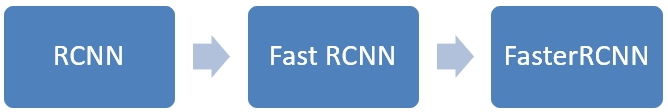
\includegraphics[width=\textwidth]{./Pictures/rcnn.jpg}	
	\caption{RCNN系列算法发展顺序}
	\label{rcnn-dev}
\end{uscfigure}

\par \noindent
他们在整个家族进化的过程中,一致暗埋了一条主线:充分利用Feature Maps的价值。

\subsubsection{R-CNN}
RCNN:(Region CNN)\cite{rcnn}可以说是利用深度学习进行目标检测的开山之作。作者Ross Girshick多次在PASCAL VOC\footnote{计算机视觉里面很大一块是在做物体的识别、检测还有分类(object recognition, detection and classification)。几乎在每一个应用领域都需要用到这三项功能,所以能否顺利的完成这三个功能,对检验一个算法的正确性和效率来说是至关重要的。所以每一个算法的设计者都会运用自己搜集到的场景图片对算法进行训练和检测,这个过程就逐渐的形成了数据集}的目标检测竞赛中折桂,2010年更带领团队获得终身成就奖。图\ref{rcnn}这个模型,利用卷积神经网络来做“目标检测”,其深远意义不言而喻。
\begin{uscfigure}
	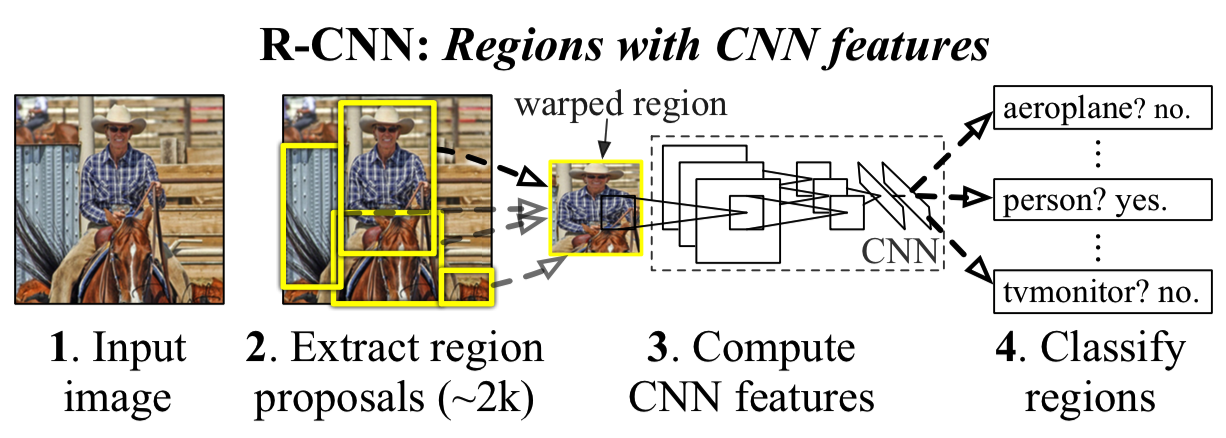
\includegraphics[width=\textwidth]{./Pictures/rcnn-regions_with_cnn_features.png}	
	\caption{RCNN算法框架}
	\label{rcnn}
\end{uscfigure}
该算法解决了目标检测中的两个关键问题:

\textbf{解决问题一、速度。}
传统的区域选择使用滑窗,每滑一个窗口检测一次,相邻窗口信息重叠高,检测速度慢。R-CNN使用一个启发式方法(Selective Search\cite{ss}),先生成候选区域再检测,降低信息冗余程度,从而提高检测速度。

\textbf{解决问题二、训练集。}
经典的目标检测算法在区域中提取人工设定的特征(Haar,HOG)。传统的手工提取特征鲁棒性差,限于如颜色、纹理等 低层次(Low level)的特征。使用CNN(卷积神经网络)提取特征,可以提取更高层面的抽象特征,从而提高特征的鲁棒性。

该方法将PASCAL VOC上的检测率从35.1\% 提升到53.7 \% ,提高了几个量级。

\textbf{算法流程:}

\line
\begin{itemize}
	\setlength{\itemsep}{0pt}
	\setlength{\parsep}{0pt}
	\setlength{\parskip}{0pt}
	\item[>] 一张图像生成1K至2K个候选区域
	\item[>] 对每个候选区域,使用深度网络提取特征
	\item[>] 特征送入每一类的SVM分类器,判别是否属于该类
	\item[>] 使用回归器精细修正候选位置	
\end{itemize}
\line

\textbf{1、候选区域生成:}使用Selective Search方法从一张图像生成约2000-3000个候选区域。基本思路如下:1、使用一种分割手段,将图像分割成小区域。2、查看现有小区域,合并可能性最高的两个区域。重复直到整张图像合并成一个区域位置。3、输出所有曾经存在过的区域,所谓候选区域。

\textbf{2、特征提取:}借鉴Hinton 2012年在Image Net上的分类网络\footnote{Hinton在2012年提出的AlexNet网络},提取特征。

\textbf{3、类别判断:}对每一类目标,使用一个线性SVM二类分类器进行判别。输入为深度网络输出的4096维特征,输出是否属于此类。由于负样本很多,使用"Hard Negative Mining"\footnote{选择正负样本的方法}方法。

\textbf{4、位置精修:}目标检测问题的衡量标准是重叠面积:许多看似准确的检测结果,往往因为候选框不够准确,重叠面积很小。故需要一个位置精修步骤。 

\subsubsection{SPP Net}
R-CNN提出后的一年,以何恺明、任少卿为首的团队发表了SPP Net:\textit{Spatial Pyramid Pooling in Deep Convolutional Networks for Visual Recognition}\cite{sppnet} ,这才是真正摸到了卷积神经网络的脉络。尽管R-CNN效果不错,但是他还有两个缺点:

\textbf{缺点一、算力冗余。}
先生成候选区域,再对区域进行卷积,这里有两个问题:其一是候选区域会有一定程度的重叠,对相同区域进行重复卷积;其二是每个区域进行新的卷积需要新的存储空间。何恺明等人意识到这个可以优化,于是把先生成候选区域再卷积,变成了先卷积后生成区域。通过“简单地”改变顺序,不仅减少存储量而且加快了训练速度。

\textbf{缺点二、图片缩放。}
无论是剪裁(Crop)还是缩放(Warp),在很大程度上会丢失图片原有的信息导致训练效果不好,如图\ref{sppnet}所示。直观的理解,把车剪裁成一个门,人看到这个门也不好判断整体是一辆车;把一座高塔缩放成一个胖胖的塔,使得机器的识别难度巨大。
\begin{uscfigure}
	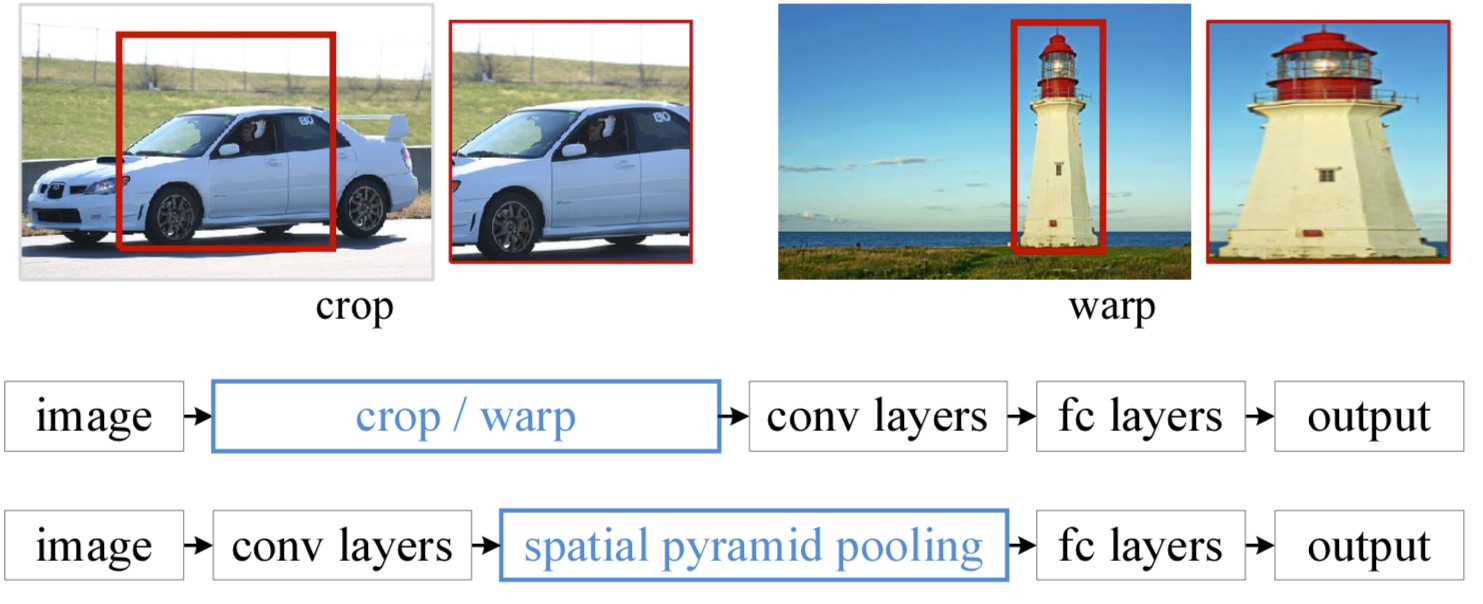
\includegraphics[width=\textwidth]{./Pictures/sppnet_crop_warp.jpg}	
	\caption{因剪裁和缩放导致视差}
	\label{sppnet}
\end{uscfigure}
何恺明等人发现了这个问题,于是思索有什么办法能不对图片进行变形,且保留原图整体信息直接进行学习。最后,他们发现问题的根源是全连接层(FC Layer)需要确定输入维度,于是他们在输入全连接层前定义一个特殊的池化层,将输入的任意尺度Feature Maps组合成特定维度的输出,这个组合可以是不同大小的拼凑,如图\ref{sppnet},我们要输入的维度 $64∗256$ ,那么我们可以这样组合 $32∗256+16∗256+8∗256+8∗256$。
\begin{uscfigure}
	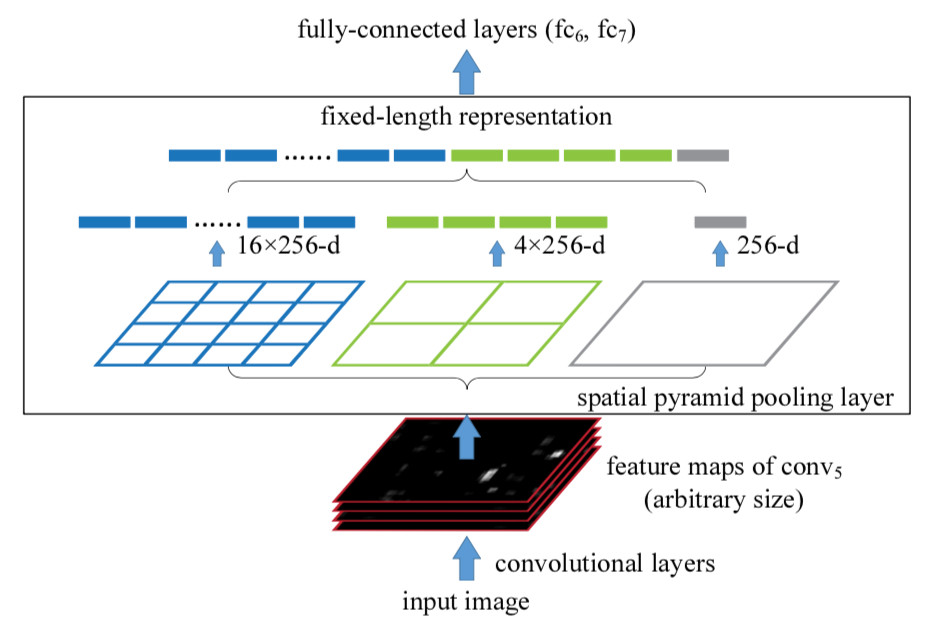
\includegraphics[width=\textwidth,]{./Pictures/sppnet_pool_layer.jpg}	
	\caption{输入维度的组合方式}
	\label{sppnet}
\end{uscfigure}
SPP Net的出现打破了常规,不仅减少了计算冗余从而提高了检测速度,更重要的是打破了固定尺寸输入这一束缚,被后面出现的算法广泛采用,其意义重大。本文基于的SSD算法就是更是从中受到启发。

\subsubsection{Fast R-CNN}
继2013年的RCNN之后,Ross Girshick在15年推出Fast RCNN\cite{fastrcnn},构思精巧,流程更为紧凑,大幅提升了目标检测的速度。在这篇论文中,引用了SPP Net的贡献 。纵观全文,最大的贡献就是将原来的串行结构改成并行结构。同样使用最大规模的网络,Fast RCNN和RCNN相比,训练时间从84小时减少为9.5小时,测试时间从47秒减少为0.32秒。在PASCAL VOC 2007上的准确率相差无几,约在66\%-67\%之间。其算法框架如图\ref{fast-rcnn}
\begin{uscfigure}
	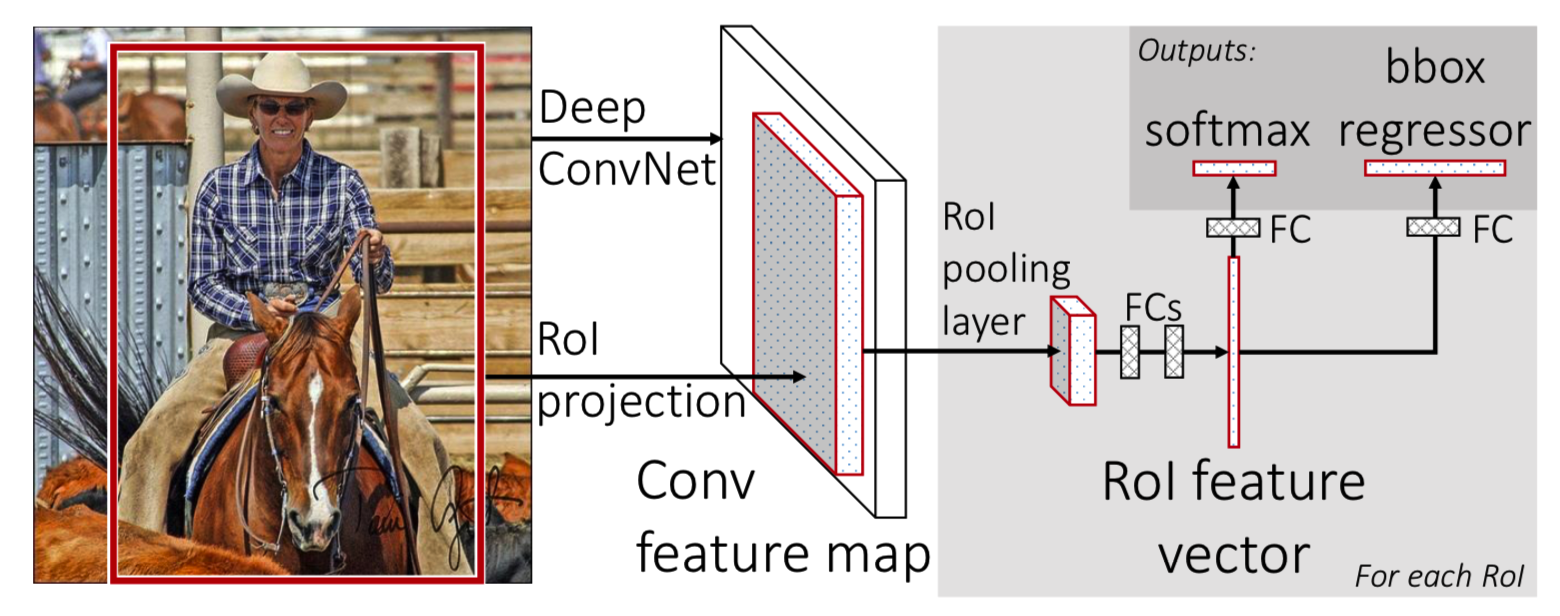
\includegraphics[width=\textwidth]{./Pictures/fast_rcnn.png}	
	\caption{Fast R-CNN算法框架}	
	\label{fast-rcnn}
\end{uscfigure}
原来的R-CNN是先对候选框区域进行分类,判断有没有物体,如果有则对Bounding Box进行精修、回归。这是一个串联式的任务,那么势必没有并联的快,所以Ross Girshick就将原有结构改成并行——在分类的同时,对Bbox进行回归。这一改变将Bbox和Clf的loss结合起来变成一个Loss一起训练,并吸纳了SPP Net的优点,最终不仅加快了预测的速度,而且提高了精度。

\textbf{算法流程:}

\line
\begin{itemize}
	\setlength{\itemsep}{0pt}
	\setlength{\parsep}{0pt}
	\setlength{\parskip}{0pt}
	\item[>] 在图像中确定1000-2000个候选框 
	\item[>] 对于每个候选框内图像块,使用深度网络提取特征
	\item[>] 对候选框中提取出的特征,使用分类器判别是否属于一个特定类
	\item[>] 对于属于某一特征的候选框,用回归器进一步调整位置
\end{itemize}
\line\\
Fast RCNN方法解决了RCNN方法三个问题:

\textbf{问题一、测试时速度慢。}RCNN一张图像内候选框之间大量重叠,提取特征操作冗余,本文将整张图像归一化后直接送入深度网络。在邻接时,才加入候选框信息,在末尾的少数几层处理每个候选框。

\textbf{问题二、训练时速度慢。}原因同问题一,在训练时,本文先将一张图像送入网络,紧接着送入从这幅图像上提取出的候选区域。这些候选区域的前几层特征不需要再重复计算。

\textbf{问题三、训练所需空间大。}RCNN中独立的分类器和加归器需要大量特征作为训练样,本文把类别判断和位置精调统一用深度网络实现,不再需要额外存储。其网络模型如图\ref{fast-rcnn-model}

\begin{uscfigure}
	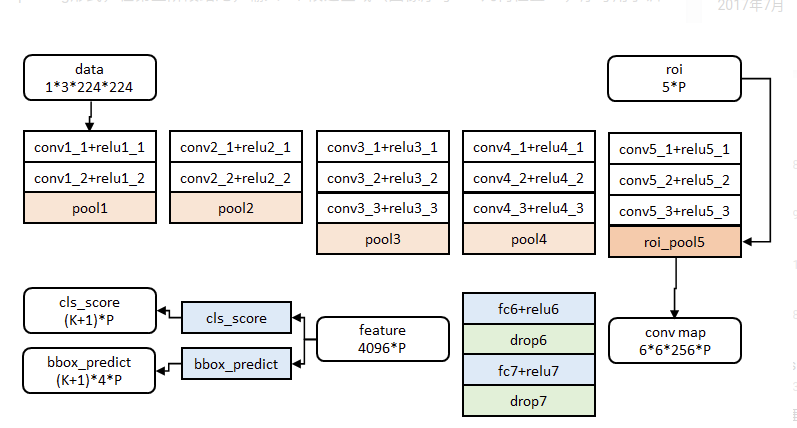
\includegraphics[width=\textwidth]{./Pictures/fast-rcnn-model.png}	
	\caption{Fast R-CNN网络模型}	
	\label{fast-rcnn-model}
\end{uscfigure}

\textbf{损失函数:}
loss\_cls层评估分类代价。由真实分类$u$对应的概率决定:
\[
	L_{cls} = - \log p_u
\]
loss\_bbox评估检测框定位代价。比较真实分类对应的预测参数$t^u$和真实平移绽放为$v$的差别:
\[
	L_{loc} = \sum_{i=1}^{4} g(t_i^u - v_i)
\]
g为Smooth L1误差,对outlier不敏感:
\begin{equation}
	g(x) = \left \{
		\begin{aligned}
		& 0.5x^2 	 & |x| < 1	\\	
		& |x| - 0.5  &otherwise
		\end{aligned}
		\right .
\end{equation}
总代价为两者加权和,如果分类为背景则不考虑定位代价:
\begin{equation}
	L = \left \{
		\begin{aligned}
		& L_{cls} + \lambda L_{loc} & u\\
		& L_{cls} 					& u
		\end{aligned}
	\right .
\end{equation}
\subsubsection{Faster R-CNN}
继RCNN,Fast RCNN之后,目标检测界的领军人物Ross Girshick团队在2015年的又一力作。简单网络目标检测速度达到17FPS,在PASCAL VOC上准确率为59.9\%;复杂网络达到5FPS,准确率78.8\%。在Faster R-CNN前,我们生产候选区域都是用的一系列启发式算法,基于Low Level特征生成区域。这样就有两个问题:

\textbf{第一个问题}每次生成区域具有不确定性,而“Two Stage”算法正是依靠生成区域的不确定性——生成大量无效区域则会造成算力的浪费、少生成区域则会漏检;

\textbf{第二个问题}是生成候选区域的算法是在CPU上运行的,而我们的训练在GPU上面,跨结构交互必定会有损效率。

那么怎么解决这两个问题呢?于是乎,任少卿等人提出了一个RPN:Region Proposal Networks的概念,利用神经网络自己学习去生成候选区域。其结构如图\ref{rpn}。
\begin{uscfigure}
	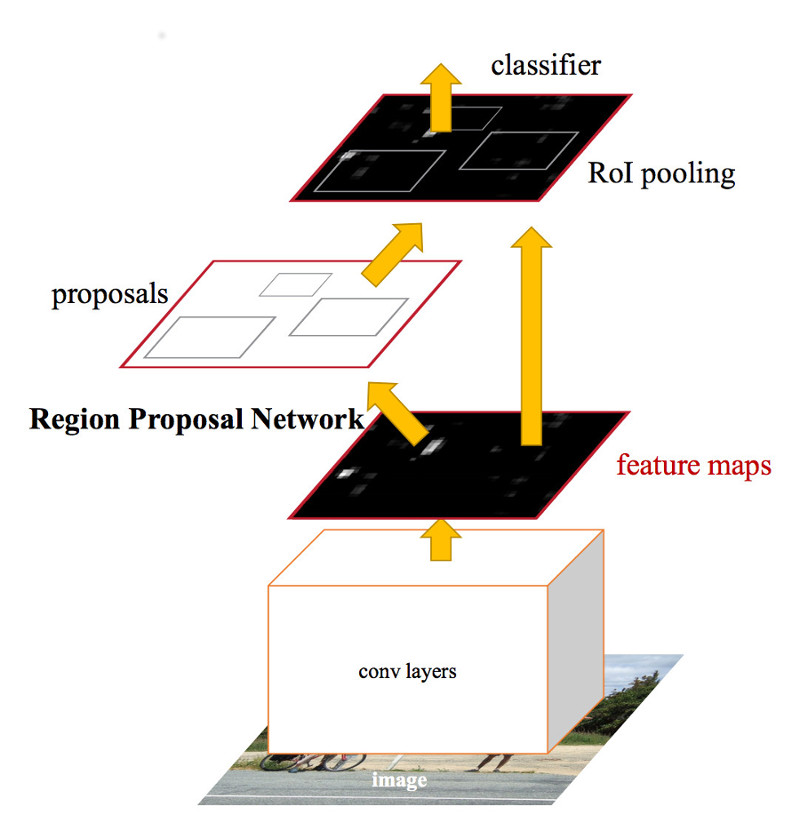
\includegraphics[width=\textwidth,height=8cm]{./Pictures/faster_rcnn.jpg}	
	\caption{Faster RCNN算法架构}	
	\label{rpn}
\end{uscfigure}
这种生成方法同时解决了上述的两个问题,神经网络可以学到更加高层、语义、抽象的特征,生成的候选区域的可靠程度大大提高;可以从上图看出RPNs和RoI Pooling共用前面的卷积神经网络——将RPNs嵌入原有网络,原有网络和RPNs一起预测,大大地减少了参数量和预测时间。在RPN中引入了anchor的概念Feature Map中每个滑窗位置都会生成k个anchors,然后判断anchor覆盖的图像是前景还是背景,同时回归Bbox的精细位置,预测的Bbox更加精确。

从RCNN到Fast RCNN,再到Faster RCNN,目标检测的四个基本步骤(候选区域生成,特征提取,分类,位置精修)终于被统一到一个深度网络框架之内。所有计算没有重复,完全在GPU中完成,大大提高了运行速度。

Faster RCNN着重解决了三个问题:

\line
\begin{itemize}
	\setlength{\itemsep}{0pt}
	\setlength{\parsep}{0pt}
	\setlength{\parskip}{0pt}
	\item[>] 如何设计区域生成网络
	\item[>] 如何训练区域生成网络
	\item[>] 如何让区域生成网络和Faster RCNN网络共享特征提取网络
\end{itemize}
\line

\textbf{区域生成网络(RPN)}

\textbf{1、特征提取:}原始特征提取(上图灰色方框)包含若干层conv+relu,直接套用ImageNet上常见的分类网络即可。本文试验了两种网络:5层的ZF\footnote{介绍一下这个网络},16层的VGG-16,具体结构不再赘述。 额外添加一个conv+relu层,输出51*39*256维特征(feature)。

\textbf{2、候选区域:}特征可以看做一个尺度51*39的256通道图像,对于该图像的每一个位置,考虑9个可能的候选窗口:三种面积{1282,2562,5122}×三种比例{1:1,1:2,2:1}。这些候选窗口称为anchors。下图示出51*39个anchor中心,以及9种anchor示例\ref{anchor}。
 
\begin{uscfigure}
	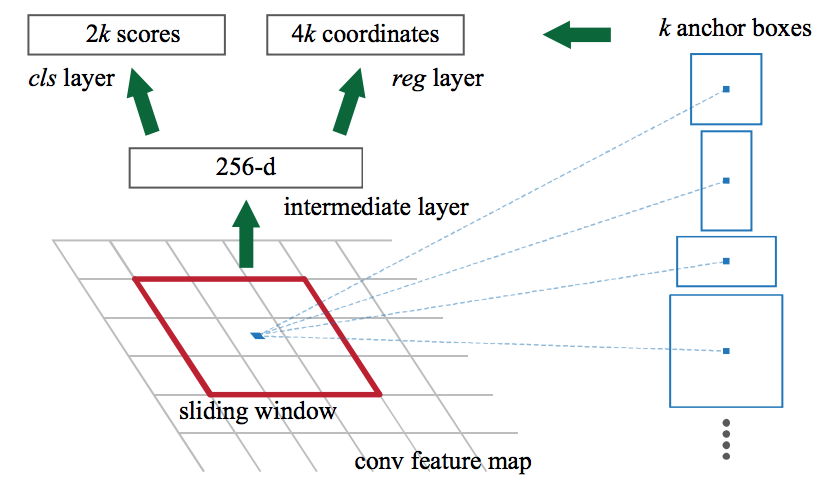
\includegraphics[width=\textwidth,height=8cm]{./Pictures/faster_rcnn_anchor.png}	
	\caption{Faster RCNN anchor示意图}	
	\label{anchor}
\end{uscfigure}

\textbf{3、窗口分类和位置精修:}分类层(cls\_score)输出每一个位置上,9个anchor属于前景和背景的概率;窗口回归层(bbox\_pred)输出每一个位置上,9个anchor对应窗口应该平移缩放的参数。 对于每一个位置来说,分类层从256维特征中输出属于前景和背景的概率;窗口回归层从256维特征中输出4个平移缩放参数。



